\documentclass{article}
% basics
\usepackage{amsfonts}
\usepackage{enumitem}
\usepackage{float}
\usepackage{graphicx}
\usepackage{hyperref} 
\usepackage[labelfont=bf]{caption}

\newtheorem{theorem}{Theorem}
\newtheorem{lemma}[theorem]{Lemma}
\newtheorem{corollary}{Corollary}[theorem]

% unique math expressions:  
\usepackage{amsmath}
\DeclareMathOperator*{\andloop}{\wedge}
\DeclareMathOperator*{\pr}{Pr}
\DeclareMathOperator*{\approach}{\longrightarrow}
\DeclareMathOperator*{\eq}{=}

% grey paper
\usepackage{xcolor}
% \pagecolor[rgb]{0.11,0.11,0.11}
% \color{white}

% embedded code sections
\usepackage{listings}
\definecolor{codegreen}{rgb}{0,0.6,0}
\definecolor{codegray}{rgb}{0.5,0.5,0.5}
\definecolor{codepurple}{rgb}{0.58,0,0.82}
\lstdefinestyle{mystyle}{
    commentstyle=\color{codegreen},
    keywordstyle=\color{magenta},
    numberstyle=\tiny\color{codegray},
    stringstyle=\color{codepurple},
    basicstyle=\ttfamily\footnotesize,
    breakatwhitespace=false,         
    breaklines=true,                 
    captionpos=b,                    
    keepspaces=true,                 
    numbers=left,                    
    numbersep=5pt,                  
    showspaces=false,                
    showstringspaces=false,
    showtabs=false,                  
    tabsize=2
}

\lstset{style=mystyle}

\begin{document}
\author{Yosef Goren \& Ori Evron}
\title{Internet Networking Homework 4 - Report}
\maketitle
\tableofcontents

\section{Running The Experiments}
The full source code to our solution in our \href{https://github.com/yosefgoren/Internet-Networking-236341}{GitHub Repository}
under the folder 'Homework4/loadBalancer'.\\
To run the simulation go to the 'loadBalancer' folder in the provided zip file or in the repo
and run the 'lb.run' script.\\
To run the emulator, go to the same folder and run \texttt{./emulator <sched\_alg\_name>}
where \texttt{<sched\_alg\_name>} should be one of '\texttt{first, rr, greedy}'.

\section{Software Design}
\subsection{Overview}
Before starting to implement the required server, we first examine
how the requred functionality can be split into distinct tasks.\\
Notably - it is possible to distinguish between the pure algorithmic task
of deciding which server should be handle each incoming request,
and the task of implementing a forwarding proxy server that can simultaniously communicate
with all of the parties involved.\\
Moveover, a modular API for the algorithmic section should allow us to
seemlessly switch between different scheduling algorithms, and to use the exact same code
within both a real proxy server, and within code that would emulate the behaviour of the system -
without actually involving any networking communications.\\

After the analysis, we conclude that our solution should have the following software modules:
\begin{itemize}
    \item \texttt{LBCore}: This module implements the various scheduling algorithms,
    and is independent of both the implementation of the actual server.\\
    This module is essentially a static library.
    \item \texttt{LBEngine}: This module accepts a scheduling algorithm and uses it implement a full-fledged
    load balancing proxy server.\\
    It is an executable.
    \item \texttt{Emulator}: This module accepts a scheduling algorithm and uses it to run an event based simulation
    of the networking system described in the homework. This simulation has a few notable advantages:
    \begin{itemize}
        \item The simulation runs almost instantly\footnote{no 'sleep', the involved code is entierly C++}.
        \item The simulation should be able to run on any platform since it does not actually make use of any socket API.
        \item It makes it easier to debug componenets used by it since it does not involve any asynchrony or multiprocessing\footnote{as opposed to the \texttt{LBEngine}}.
    \end{itemize}
\end{itemize}
\begin{center}
    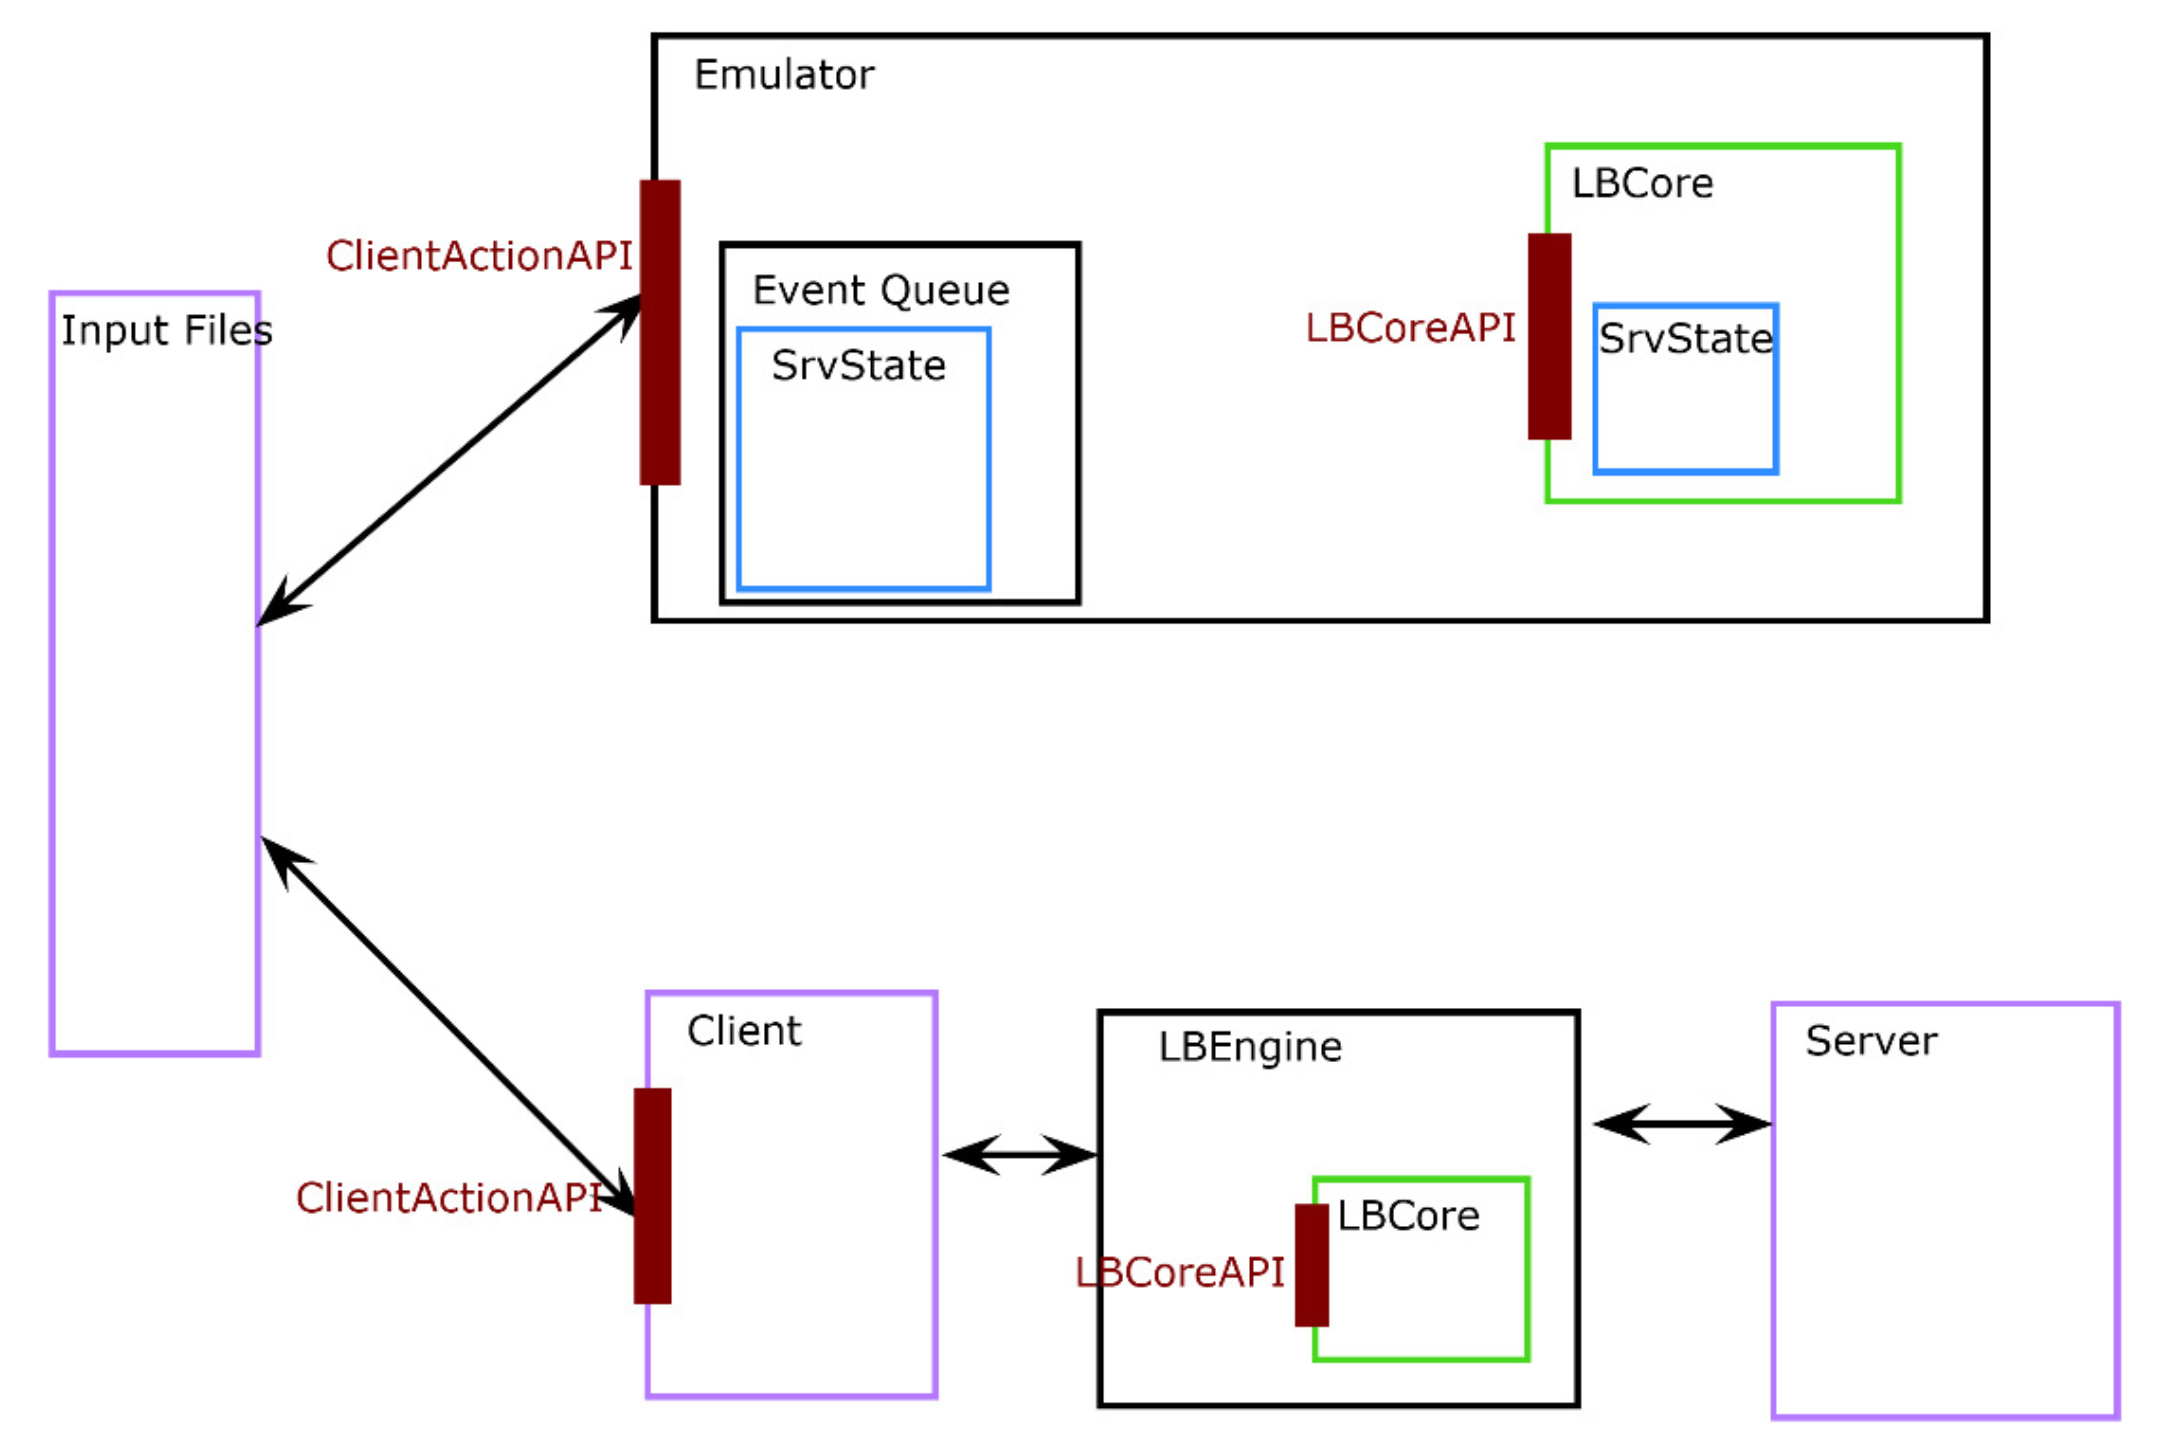
\includegraphics[width=1.2\textwidth]{design_graph.png}
\end{center}

\subsection{Design Stages}
In order to progressively implement our design we came up with the following incremental stages:
\begin{enumerate}
    \item Define the API for \texttt{LBCore}.
    \item Create a proof-of-concept application
    \footnote{can be found under \texttt{loadBalancer/SockHelloWorld}}
    to experiment with using the Linux socket API for our purposes.
    \item Create \texttt{LBEngine}.
    \item Create a basic implementation of \texttt{LBCore} with trivial algorithm
    \footnote{at this point we can debug \texttt{LBEngine}}.
    \item Create \texttt{Emulator}.
    \item Design and implement better scheduling algorithms (\texttt{LBCore}).
    \item Test performance of the schedulers using the Emulator.
\end{enumerate}

\section{Load Balancing Engine}
\subsection{Socket Manager}
The \texttt{SocketManager}
\footnote{can be found at \texttt{loadBalancer/LBEngine/LBEngine.cpp}}
played a crucial role in managing the multitude of sockets in our code.
Specifically, we needed to maintain three active sockets to the servers,
alongside a dynamically changing number of sockets to the clients.\\
To achieve this, the Socket Manager maintained a list of sockets for each working server.
Upon receiving a finish signal from a working server, we could retrieve the corresponding socket from the Socket Manager.
This socket was then used to send the finish signal to the client before closing the socket.\\
By utilizing the Socket Manager, we could ensure that all sockets were appropriately closed once we had completed our tasks.
This streamlined approach helped us manage the complex
socket interactions efficiently and maintain proper control over the communication process.


\subsection{Async Communications}
The hardest technical problem we have had to face was giving 
\texttt{LBEngine} the ability to asynchronously communicate with both the servers
and the clients.\\
The Engine has to main types of communication sockets:
\begin{enumerate}
    \item Worker Sockets: These sockets are used to communicate between the proxy server (a.k.a \texttt{LBEngine})
    and each of the worker servers. These connections are established once when the proxy server starts running and
    continue untill it is done.
    \item Client Sockets: These sockets are used to communicate between the proxy server and the
    end clients. For each request from a client - a new connection is established - which lasts which the request is being handled.
    Once a response is produced by a worker - that response is sent back over the session - and the session is closed.
\end{enumerate}
In order to be able to handle both types of requests from a single process - we have implemented
a main loop that continuously checks for either a new incoming client connection - or a new response message from
one of the worker servers. If either one is sent - it is handled by the proxy server in that same iteration of the main loop.\\
In order to be able to keep track of which response should be returned to which client
\footnote{since this information is not contained within the response messages from the workers} -
the proxy servers saves a fifo queue of client socket id's for each of the worker servers.

\section{Emulator}
\subsection{Overview}
As mentioned previously - the emulator is event based, and does not
involve any actual networking communications.
\subsection{Event Types}
There are two possible events in our simulation:
\begin{enumerate}
    \item \texttt{clientRequestEvent}: This event emulates the behaviour of a client makeing a new request to the proxy server.
    It causes a later event of type \texttt{serverResponseEvent}.
    \item \texttt{serverResponseEvent}: This event emulates a server sending a response back to the proxy server.
    If the associated client has any more requests - it will trigger an immidiate event of type \texttt{clientRequestEvent}.
\end{enumerate}
\subsection{Event Queue}
The event queue is initialized with an event of type \texttt{clientRequestEvent}
from each of the clients (with a non-empty requests list).\\
The simulation lasts as long as there are any new events to pull from the evnet queue.

\section{Scheduling Algorithms}
\subsection{Always First Worker}
Initially, we attempted to direct all client requests to the first worker server, which, of-course resulted very poor performance.

\subsection{Round Robin}
We then proceeded to implement a round-robin approach to evaluate its effectiveness.
The round-robin mechanism involved initializing a counter (modulus 3) to 0.\\
Each request was dispatched to a worker server using the current value of the counter, after which the counter was incremented.\\
The performance achieved using this round-robin approach was comparable to the performance of the code provided by the course staff.

\subsection{Greedy}
Upon further exploration, we discovered that employing a greedy algorithm proved to be the most effective solution for our problem.
Our algorithm treats each client's request as if it were the last and calculates the optimal server to dispatch it to.
By doing so, we aim to complete the execution of all requests as quickly as possible, optimizing the overall performance of the system.

\section{Results}
As previously mentioned, our experiments with the greedy algorithm yielded the best results.
In certain runs, we observed that it outperformed our round-robin approach by a factor of two,\\
resulting in significantly faster execution times.

\end{document}